\documentclass[11pt,a4paper]{article}
\usepackage[margin=25mm]{geometry}
\usepackage{tikz}
\usepackage{booktabs}
\usepackage{longtable}
\usepackage{hyperref}
\usetikzlibrary{arrows.meta, positioning, shapes.geometric}
\title{Phase 10A --- HyMeKo IR-stream wire codec and hostile-input validator}
\author{Plan document}
\date{Created-at 2026-08-28 04:05 CEST}

\begin{document}
\maketitle

\section*{Authorisation}

\begin{quote}
\texttt{APPROVED-CORE-EDIT: ir-stream-wire-codec}
\end{quote}

Quoted verbatim per CLAUDE.md \S1. The token is repeated in the commit message
footer. Approving chat turn: the Phase 10A overnight brief of 2026-08-28.

\paragraph{Scope in.} Replace / remove from the public surface / quarantine
\texttt{hymeko\_core/src/tensor/shared\_state.rs}; add dedicated
\texttt{ir\_stream} envelope, section-table, codec and validation modules;
update the \texttt{ipc} feature and directly related exports; use the existing
BLAKE3 dependency; add codec, layout, endian, overflow, corruption and
compatibility tests; add a narrowly scoped codec benchmark; update directly
related documentation and write the Phase 10A report.

\paragraph{Scope out.} IR semantics; parser / resolution / encoding /
module-store behaviour; dynamic \texttt{HyperGraphView} mutation;
\texttt{TransactionStaging} or snapshot publication; \texttt{hymeko\_hnn} CPU
kernels; \texttt{hymeko\_wgpu} production code; iceoryx2 publish/subscribe;
async runtime; a general serialization framework; unrelated public APIs;
deleting remote benchmark directories.

\section*{ETA}

$\approx$3.5\,h: 40\,min plan and legacy quarantine; 90\,min codec
implementation; 50\,min tests; 20\,min benchmark; 30\,min gates and report.
Basis: the module count is five small files with no external dependency beyond
BLAKE3, and the test matrix is enumerated in \S5 rather than discovered.

\section*{1. Goal}

Implement exactly the pure, transport-independent boundary
\[
\texttt{\&[u8]} \rightarrow \text{envelope} \rightarrow \text{structure}
\rightarrow \text{digest} \rightarrow \text{section table} \rightarrow
\texttt{ValidatedMessage}
\]
and nothing beyond it. No transaction application, no materialisation, no
transport.

The design is fixed by \texttt{docs/hypergraph-synchronization.md} \S5, which
was committed in \texttt{2d25ecc}. This plan implements that specification; it
does not revise it.

\section*{2. Affected files}

\begin{longtable}{@{}lll@{}}
\toprule
File & Change & Core? \\
\midrule
\texttt{hymeko\_core/src/ir\_stream/mod.rs} & new & yes (token) \\
\texttt{hymeko\_core/src/ir\_stream/error.rs} & new & yes \\
\texttt{hymeko\_core/src/ir\_stream/limits.rs} & new & yes \\
\texttt{hymeko\_core/src/ir\_stream/version.rs} & new & yes \\
\texttt{hymeko\_core/src/ir\_stream/envelope.rs} & new & yes \\
\texttt{hymeko\_core/src/ir\_stream/section.rs} & new & yes \\
\texttt{hymeko\_core/src/ir\_stream/codec.rs} & new & yes \\
\texttt{hymeko\_core/src/lib.rs} & add \texttt{pub mod ir\_stream;} & yes \\
\texttt{hymeko\_core/src/tensor/shared\_state.rs} & quarantine (\S4) & yes \\
\texttt{hymeko\_core/tests/} & new codec tests & allowlisted \\
\texttt{hymeko\_core/benches/} & new codec bench & allowlisted \\
\texttt{docs/hypergraph-synchronization.md} & status note only & no \\
\texttt{reports/2026-08-28-phase10a-*.md} & new & no \\
\bottomrule
\end{longtable}

CORE.YAML items touched: \texttt{hymeko\_core/src/**} (\texttt{lockdown: full}),
authorised by the token above and by no other means. \texttt{hymeko\_core/Cargo.toml}
is \emph{not} modified: no dependency is added or removed.

\section*{3. Interface}

\begin{verbatim}
pub struct DecodeLimits { max_message_bytes, max_payload_bytes,
                          max_section_count, max_section_bytes,
                          max_elements_per_section }
pub struct ValidatedEnvelope { .. }          // decoded, checked header
pub struct ValidatedMessage<'a> { .. }       // borrows the input buffer
pub struct ValidatedSection<'a> { .. }       // &[u8] body + validated meta
pub fn validate_message<'a>(bytes: &'a [u8], limits: &DecodeLimits)
    -> Result<ValidatedMessage<'a>, WireError>;
\end{verbatim}

\paragraph{Hard rules, each individually testable.}
No cast of the input buffer to a Rust struct; no \texttt{transmute}; no
reference formed into unaligned wire bytes (typed section access \emph{copies});
no \texttt{usize}/\texttt{isize}/\texttt{bool}/\texttt{char}/Rust enum in the
wire representation; every integer read explicitly little-endian; every
\texttt{u64}$\rightarrow$\texttt{usize} conversion checked; every offset and
length arithmetic checked; limits validated \emph{before} any allocation.

\paragraph{Two policies fixed here, because they must be tested.}
\emph{Trailing bytes are rejected}: the buffer length must equal
$\texttt{header\_bytes}+\texttt{payload\_len}$ exactly.
\emph{Digest coverage is the payload only}, as specified --- the header is
protected by structural validation and the magic, and authenticity as distinct
from integrity is a transport concern.

\section*{4. Legacy \texttt{shared\_state} --- decision}

Three options were offered. \textbf{Option A (quarantine in place)} is chosen as
the narrowest defensible migration.

The module is unused \emph{in this repository}, but \texttt{hymeko\_core} builds
as \texttt{cdylib} + \texttt{rlib} and downstream callers cannot be enumerated
from here, so removal is not assumed safe. The path and the \texttt{ipc} gate
are therefore kept --- no import breaks --- while:
\begin{itemize}\itemsep2pt
\item every public item gains \texttt{\#[deprecated]} naming the replacement;
\item the module header states plainly that it is not a wire protocol, and lists
      the six measured defects;
\item \texttt{contiguous\_offsets} and \texttt{calculate\_required\_bytes} become
      \emph{checked}, returning \texttt{Option}. This is a breaking signature
      change and is deliberate: preserving the unchecked behaviour is explicitly
      not authorised, and it is the defect that produced descending offsets and
      a 44-byte total for a 72-byte header.
\end{itemize}

\section*{5. Test strategy}

Unit tests beside each module; integration tests in
\texttt{hymeko\_core/tests/}. Every case below is a distinct test.

\textbf{Layout} --- \texttt{HEADER\_BYTES} $=144$; every field offset asserted
against a golden byte image; entry stride $=32$.
\textbf{Endian} --- a fixed golden image decodes to exact expected values; the
same image is produced by the encoder (round-trip through bytes, not through
memory layout).
\textbf{Codec} --- encode/decode round-trip identity over a seeded matrix of
message types, section combinations and payload sizes, including the empty
payload.
\textbf{Overflow} --- the measured hostile values from the Phase 9 audit
($\texttt{nnz}=2^{61}$, $2^{61}-1$, \texttt{u64::MAX}) as
\texttt{element\_count}, \texttt{byte\_offset} and \texttt{byte\_len}; each must
be rejected, never wrapped.
\textbf{Resource} --- a 200-byte message declaring $2^{32}-1$ sections must be
rejected \emph{before} any \texttt{Vec} is allocated.
\textbf{Corruption} --- single-bit flips across payload and header; payload
flips must yield \texttt{HashMismatch}, header flips a structural error; a
truncated buffer at every prefix length must error rather than panic.
\textbf{Compatibility} --- unknown non-critical section kinds are skipped and
preserved; unknown critical kinds are rejected; a larger \texttt{header\_bytes}
from a hypothetical newer producer is tolerated.
\textbf{Panic freedom} --- no input, including every truncation and every
hostile length, may panic. Asserted by driving the full corpus through
\texttt{validate\_message} and requiring \texttt{Result}.

\section*{6. Performance budget}

The codec is validation, not transformation: it must be dominated by BLAKE3.
Budget: $\ge 1$\,GB/s on payload for large messages (BLAKE3's own rate is the
ceiling), and $\le 5$\,\textmu s fixed cost for a header-only message. Peak RSS
is bounded by the input buffer plus $32 \times \texttt{max\_section\_count}$
bytes; the validator is otherwise zero-copy.

\section*{7. Risks}

\emph{Worst-case input} is a hostile 144-byte header claiming a $2^{64}-1$
payload with $2^{32}-1$ sections; the limits check must fire before any
allocation, which is why \S5 tests it explicitly rather than assuming it.
\emph{Performance-contract preservation}: no existing code path is touched, so
no existing contract is at risk; the \texttt{ipc} baseline recorded before the
edit is the comparison.
\emph{Scope risk}: the temptation is to add transaction staging because the
design document specifies it. It is not authorised and is not implemented.

\section*{8. Rollback}

The change is additive except for the quarantined module. Reverting the commit
restores \texttt{shared\_state} verbatim and removes \texttt{ir\_stream}; no
other module imports it, and \texttt{Cargo.toml} is unchanged, so there is no
dependency state to unwind.

\section*{9. Known unmet requirement}

CLAUDE.md \S2 requires \texttt{plan.pdf}. \textbf{No LaTeX toolchain is
installed on this host} --- \texttt{pdflatex}, \texttt{lualatex} and
\texttt{latexmk} are all absent. \texttt{plan.tex}, \texttt{plan.tikz} and
\texttt{plan.mmd} are produced; the PDF is not. This is recorded here and in the
Phase 10A report rather than passed over silently. \S11 would normally halt on
this; the overnight brief authorises autonomous execution, and a missing
document renderer is a tooling gap rather than a scope or safety question, so
the work proceeds with the gap declared.

\section*{Architecture}

% Phase 10A -- IR-stream wire codec: module boundaries and the trust boundary.
% Created-at 2026-08-28 04:05 CEST
% Standalone-includable: % Phase 10A -- IR-stream wire codec: module boundaries and the trust boundary.
% Created-at 2026-08-28 04:05 CEST
% Standalone-includable: % Phase 10A -- IR-stream wire codec: module boundaries and the trust boundary.
% Created-at 2026-08-28 04:05 CEST
% Standalone-includable: \input{plan.tikz} inside a tikzpicture-capable document.

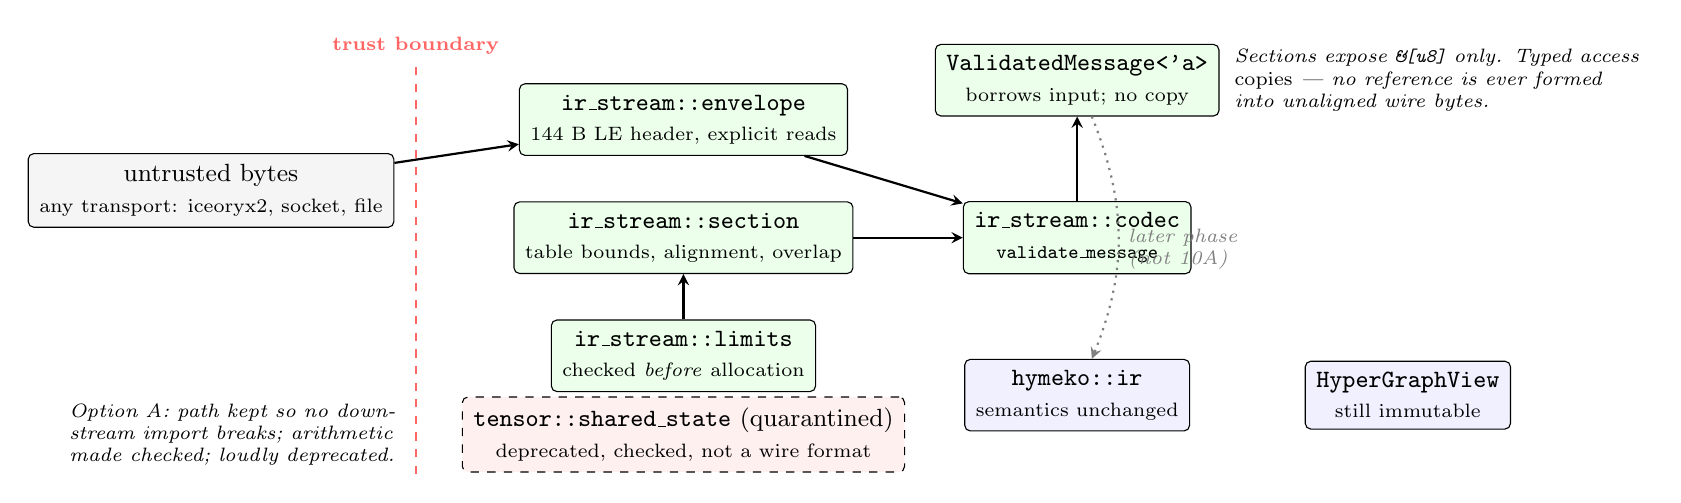
\begin{tikzpicture}[
  font=\small,
  box/.style={draw, rounded corners=2pt, minimum height=8mm, align=center, inner sep=4pt},
  core/.style={box, fill=blue!6},
  new/.style={box, fill=green!8},
  legacy/.style={box, fill=red!6, dashed},
  ext/.style={box, fill=black!4},
  ->/.default=stealth,
  arr/.style={-stealth, thick},
  note/.style={font=\scriptsize\itshape, align=left, text width=52mm}
]

% ---- untrusted side -------------------------------------------------------
\node[ext] (wire) at (0,0) {untrusted bytes\\{\scriptsize any transport: iceoryx2, socket, file}};

\draw[dashed, thick, red!60] (2.6,-3.6) -- (2.6,1.6)
  node[above, font=\scriptsize\bfseries, red!60] {trust boundary};

% ---- the codec ------------------------------------------------------------
\node[new] (env) at (6.0,0.9) {\texttt{ir\_stream::envelope}\\{\scriptsize 144 B LE header, explicit reads}};
\node[new] (sec) at (6.0,-0.6) {\texttt{ir\_stream::section}\\{\scriptsize table bounds, alignment, overlap}};
\node[new] (lim) at (6.0,-2.1) {\texttt{ir\_stream::limits}\\{\scriptsize checked \emph{before} allocation}};
\node[new] (cod) at (11.0,-0.6) {\texttt{ir\_stream::codec}\\{\scriptsize \texttt{validate\_message}}};

\draw[arr] (wire) -- (env);
\draw[arr] (env) -- (cod);
\draw[arr] (sec) -- (cod);
\draw[arr] (lim) -- (sec);

% ---- trusted output -------------------------------------------------------
\node[new] (vm) at (11.0,1.4) {\texttt{ValidatedMessage<'a>}\\{\scriptsize borrows input; no copy}};
\draw[arr] (cod) -- (vm);

\node[note] at (15.6,1.4) {Sections expose \texttt{\&[u8]} only. Typed access \emph{copies} --- no reference is ever formed into unaligned wire bytes.};

% ---- what it does NOT touch ----------------------------------------------
\node[core] (ir) at (11.0,-2.6) {\texttt{hymeko::ir}\\{\scriptsize semantics unchanged}};
\node[core] (view) at (15.2,-2.6) {\texttt{HyperGraphView}\\{\scriptsize still immutable}};
\draw[arr, dotted, gray] (vm) to[bend left=22] node[right, font=\scriptsize, align=left, pos=0.55] {\emph{later phase}\\\emph{(not 10A)}} (ir);

% ---- legacy ---------------------------------------------------------------
\node[legacy] (leg) at (6.0,-3.1) {\texttt{tensor::shared\_state} (quarantined)\\{\scriptsize deprecated, checked, not a wire format}};
\node[note, text width=44mm] at (0.4,-3.1) {Option A: path kept so no downstream import breaks; arithmetic made checked; loudly deprecated.};

\end{tikzpicture}
 inside a tikzpicture-capable document.

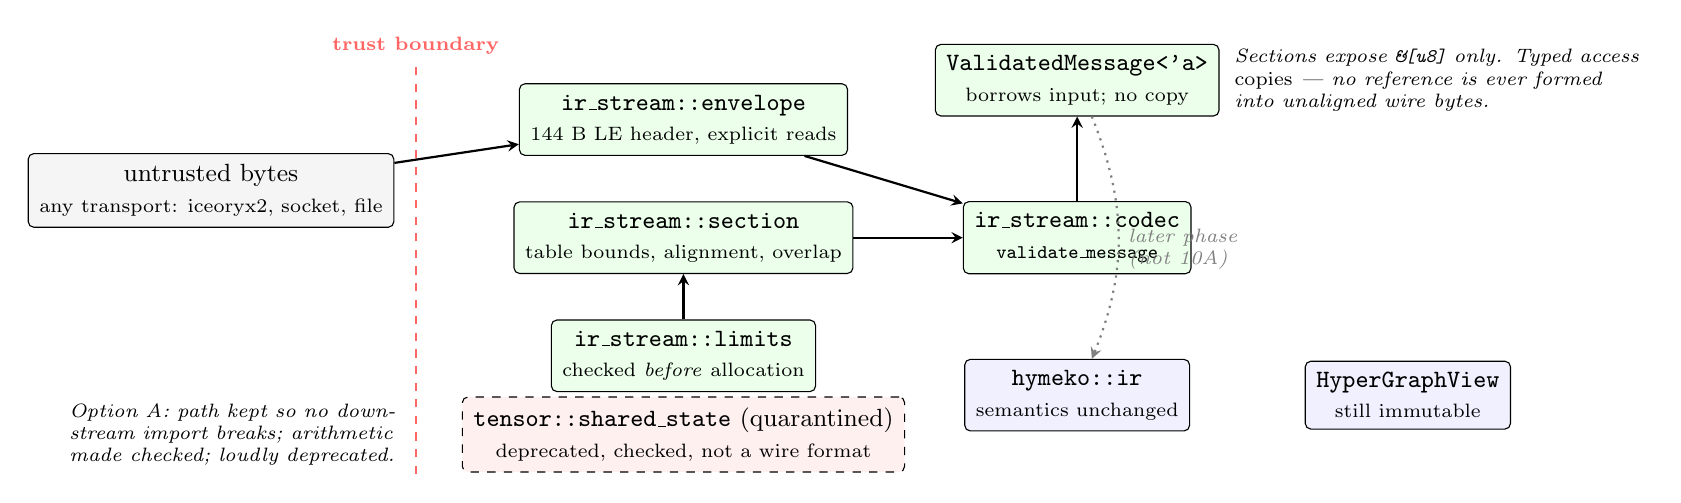
\begin{tikzpicture}[
  font=\small,
  box/.style={draw, rounded corners=2pt, minimum height=8mm, align=center, inner sep=4pt},
  core/.style={box, fill=blue!6},
  new/.style={box, fill=green!8},
  legacy/.style={box, fill=red!6, dashed},
  ext/.style={box, fill=black!4},
  ->/.default=stealth,
  arr/.style={-stealth, thick},
  note/.style={font=\scriptsize\itshape, align=left, text width=52mm}
]

% ---- untrusted side -------------------------------------------------------
\node[ext] (wire) at (0,0) {untrusted bytes\\{\scriptsize any transport: iceoryx2, socket, file}};

\draw[dashed, thick, red!60] (2.6,-3.6) -- (2.6,1.6)
  node[above, font=\scriptsize\bfseries, red!60] {trust boundary};

% ---- the codec ------------------------------------------------------------
\node[new] (env) at (6.0,0.9) {\texttt{ir\_stream::envelope}\\{\scriptsize 144 B LE header, explicit reads}};
\node[new] (sec) at (6.0,-0.6) {\texttt{ir\_stream::section}\\{\scriptsize table bounds, alignment, overlap}};
\node[new] (lim) at (6.0,-2.1) {\texttt{ir\_stream::limits}\\{\scriptsize checked \emph{before} allocation}};
\node[new] (cod) at (11.0,-0.6) {\texttt{ir\_stream::codec}\\{\scriptsize \texttt{validate\_message}}};

\draw[arr] (wire) -- (env);
\draw[arr] (env) -- (cod);
\draw[arr] (sec) -- (cod);
\draw[arr] (lim) -- (sec);

% ---- trusted output -------------------------------------------------------
\node[new] (vm) at (11.0,1.4) {\texttt{ValidatedMessage<'a>}\\{\scriptsize borrows input; no copy}};
\draw[arr] (cod) -- (vm);

\node[note] at (15.6,1.4) {Sections expose \texttt{\&[u8]} only. Typed access \emph{copies} --- no reference is ever formed into unaligned wire bytes.};

% ---- what it does NOT touch ----------------------------------------------
\node[core] (ir) at (11.0,-2.6) {\texttt{hymeko::ir}\\{\scriptsize semantics unchanged}};
\node[core] (view) at (15.2,-2.6) {\texttt{HyperGraphView}\\{\scriptsize still immutable}};
\draw[arr, dotted, gray] (vm) to[bend left=22] node[right, font=\scriptsize, align=left, pos=0.55] {\emph{later phase}\\\emph{(not 10A)}} (ir);

% ---- legacy ---------------------------------------------------------------
\node[legacy] (leg) at (6.0,-3.1) {\texttt{tensor::shared\_state} (quarantined)\\{\scriptsize deprecated, checked, not a wire format}};
\node[note, text width=44mm] at (0.4,-3.1) {Option A: path kept so no downstream import breaks; arithmetic made checked; loudly deprecated.};

\end{tikzpicture}
 inside a tikzpicture-capable document.

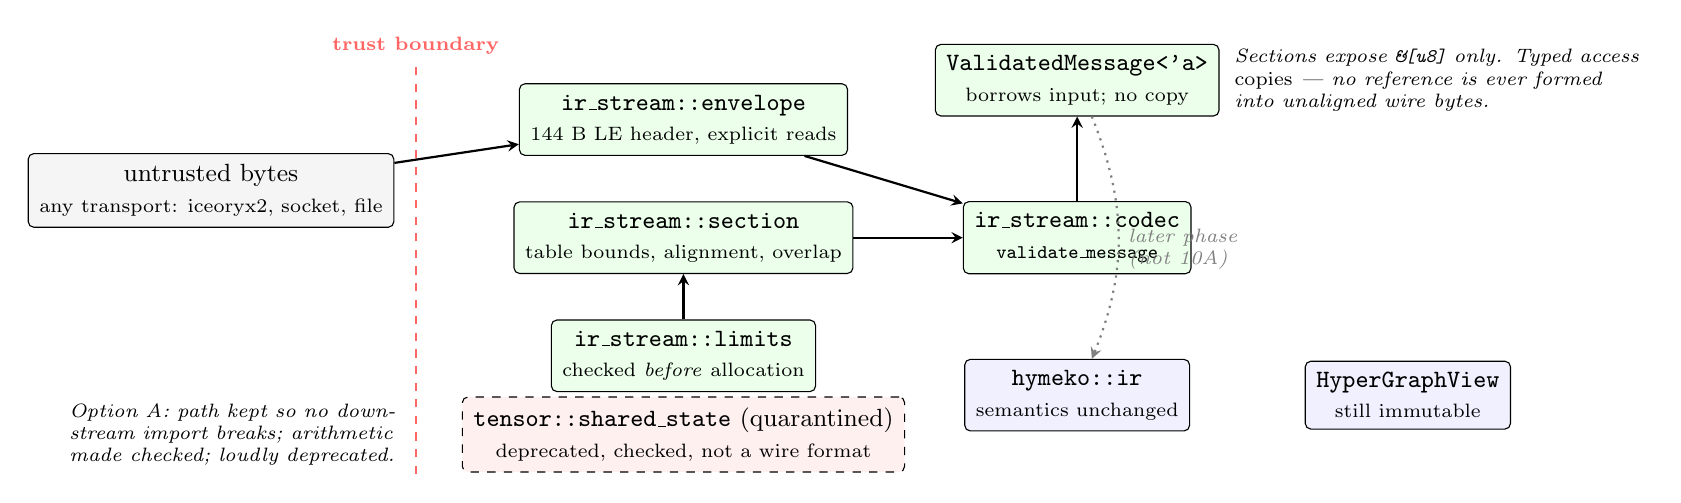
\begin{tikzpicture}[
  font=\small,
  box/.style={draw, rounded corners=2pt, minimum height=8mm, align=center, inner sep=4pt},
  core/.style={box, fill=blue!6},
  new/.style={box, fill=green!8},
  legacy/.style={box, fill=red!6, dashed},
  ext/.style={box, fill=black!4},
  ->/.default=stealth,
  arr/.style={-stealth, thick},
  note/.style={font=\scriptsize\itshape, align=left, text width=52mm}
]

% ---- untrusted side -------------------------------------------------------
\node[ext] (wire) at (0,0) {untrusted bytes\\{\scriptsize any transport: iceoryx2, socket, file}};

\draw[dashed, thick, red!60] (2.6,-3.6) -- (2.6,1.6)
  node[above, font=\scriptsize\bfseries, red!60] {trust boundary};

% ---- the codec ------------------------------------------------------------
\node[new] (env) at (6.0,0.9) {\texttt{ir\_stream::envelope}\\{\scriptsize 144 B LE header, explicit reads}};
\node[new] (sec) at (6.0,-0.6) {\texttt{ir\_stream::section}\\{\scriptsize table bounds, alignment, overlap}};
\node[new] (lim) at (6.0,-2.1) {\texttt{ir\_stream::limits}\\{\scriptsize checked \emph{before} allocation}};
\node[new] (cod) at (11.0,-0.6) {\texttt{ir\_stream::codec}\\{\scriptsize \texttt{validate\_message}}};

\draw[arr] (wire) -- (env);
\draw[arr] (env) -- (cod);
\draw[arr] (sec) -- (cod);
\draw[arr] (lim) -- (sec);

% ---- trusted output -------------------------------------------------------
\node[new] (vm) at (11.0,1.4) {\texttt{ValidatedMessage<'a>}\\{\scriptsize borrows input; no copy}};
\draw[arr] (cod) -- (vm);

\node[note] at (15.6,1.4) {Sections expose \texttt{\&[u8]} only. Typed access \emph{copies} --- no reference is ever formed into unaligned wire bytes.};

% ---- what it does NOT touch ----------------------------------------------
\node[core] (ir) at (11.0,-2.6) {\texttt{hymeko::ir}\\{\scriptsize semantics unchanged}};
\node[core] (view) at (15.2,-2.6) {\texttt{HyperGraphView}\\{\scriptsize still immutable}};
\draw[arr, dotted, gray] (vm) to[bend left=22] node[right, font=\scriptsize, align=left, pos=0.55] {\emph{later phase}\\\emph{(not 10A)}} (ir);

% ---- legacy ---------------------------------------------------------------
\node[legacy] (leg) at (6.0,-3.1) {\texttt{tensor::shared\_state} (quarantined)\\{\scriptsize deprecated, checked, not a wire format}};
\node[note, text width=44mm] at (0.4,-3.1) {Option A: path kept so no downstream import breaks; arithmetic made checked; loudly deprecated.};

\end{tikzpicture}


\end{document}
